\section{Evaluation}
\label{sec:evaluation}
% Memória
% Latência
% Tempo de reconfiguração

%The reprogramming structure formed by \ELUS{} and the dissemination protocol were evaluated in terms of memory consumption, latency of sending data across the network and reconfiguration time.
The infrastructure was evaluated in terms of memory consumption, latency of sending data across the network and reconfiguration time.
%These tests were performed using Mica2\footnote{Sensor node which has an ATMega128 microcontroller, 4KB RAM, 128KB of flash memory, 4KB of EEPROM and radio communication.} nodes.
These tests were performed using Mica2 nodes.
The system was generated with the GNU compiler g++ 4.0.2 and memory consumption measured using the GNU \textit{objdump} 2.16.1 tool.
Latency and reconfiguration times were measured by the timer of the microcontroller.

\subsection{Memory}
Table~\ref{tab:mem} shows the memory consumption of all the framework's elements. For this test, the reconfiguration support was enabled for a component that contains 4 methods. The dissemination protocol occupies 2536 bytes in code area and 21 bytes in the uninitialized data. It is important to notice that a buffer is created dynamically when the new code is received, and its size depends on the size of the update. The \ELUS{} framework consumes 1648 bytes of code, 26 bytes of data and 68 bytes of uninitialized data due to the variables and tables required to store objects and methods.
\begin{table}
\centering
\scriptsize{
%\caption{Consumo de memória da estrutura: \ELUS{} e protocolo de disseminação.}
\caption{Memory consumption of the structure: \ELUS{} and dissemination protocol.}
\begin{tabular}{|c|c|c|c|c|}\hline
\textbf{Structure} & \multicolumn{4}{c|}{\textbf{Section size (bytes)}} \cr
\cline{2-5}
\textbf{Elements} & \textbf{.text} & \textbf{.data} & \textbf{.bss} & \textbf{.bootloader} \cr
\hline
\textbf{Dissemination Protocol} & 2536 & 0 & 21 & 0 \cr\hline
\textbf{\textsc{Reconfigurator}} & 166 & 0 & 4 & 0 \cr\hline
\textbf{AVR Code Manager} & 36 & 0 & 0 & 416 \cr\hline
\textbf{\ELUS{}} & 1648 & 26 & 68 & 0 \cr\hline
\hline
\textbf{Total} & 4386 & 26 & 93 & 416 \cr
\hline
\end{tabular}
\label{tab:mem}
}
\end{table}

Table~\ref{tab:elusMem} shows the memory consumption required by \ELUS{} when a novel component is added to the system. The methods \texttt{Create}, \texttt{Destroy} and \texttt{Update} represent the constructor, destructor and update method for the component, and must always be present. Each component also requires a semaphore to control its exclusive access and prevent an update while the code is running. The minimum consumption to a new component added to the framework is composed of the constructor, destructor, \texttt{Update} method and a method without parameters and without returning value.% , and is 664 bytes of code and 26 bytes of data.
\begin{table}
\centering
\scriptsize{
%\caption{Consumo de memória do \ELUS{} ao habilitar o suporte à reconfiguração em um componente.}
\caption{Memory consumption of \ELUS{} to enable support for a reconfiguration component.}
\begin{tabular}{|c|c|c|}\hline
\textbf{Framework} & \multicolumn{2}{c|}{\textbf{Section Size (bytes)}} \cr
\cline{2-3}
\textbf{Methods} & \textbf{.text} & \textbf{.data} \cr
\hline
Create & 178 & 0 \cr\hline
Destroy & 136 & 0 \cr\hline
Method without parameter & 90 & 0 \cr
and return value & & \cr\hline
Method with parameter & 94 & 0 \cr
and without return value & & \cr\hline
Method without parameter & 104 & 0 \cr
and with return value & & \cr\hline
Method with parameter & 122 & 0 \cr
and return value & & \cr\hline
Update & 260 & 0 \cr\hline
Dispatcher & 0 & 2 X (n. of methods) \cr\hline
Semaphore & 0 & 18 \cr\hline
\hline
\textbf{Minimum size} & 664 & 26 \cr
\hline
\end{tabular}
\label{tab:elusMem}
}
\end{table}
%Equation~\ref{for:size} summarizes the extra cost of memory. The size of a component "C" is the sum of the size of all methods, as shown in Table~\ref{tab:elusMem}, with the size of implementation of component's methods. Also, the size of methods \texttt{Create}, \texttt{Destroy} and \texttt{Update} must be added to this sum. The data size is the sum of component data, values of \texttt{Dispatcher} and \texttt{Semaphore} used by \ELUS{}.
Equation~\ref{for:size} summarizes the extra cost of memory.
\begin{equation}
\label{for:size}
Size_{c} = \sum_{i=1}^n (Method_{i}) + Create + Destroy + Update
\end{equation} 
%The proposed specialization through void pointers showed positive results for memory consumption.
Using the specialization through void pointers it was possible to reduce consumption of approximately 1.2KB (more than 50\%). Currently the minimum size for a new component of the system is 664KB instead of 1.6KB from the previous ELUS implementation \cite{Gracioli:2010}.

\subsection{Latency}
%Foram utilizadas duas topologias para medir a latência do protocolo de disseminação, ilustradas na Figura \ref{fig:topology}: (a) a estação base possui comunicação com todos os nodos, (b) a estação base não possui comunicação com um nodo, que está ao alcance dos outros. Em ambas topologias repetiu-se o processo de disseminação vinte vezes, de forma a atualizar um método de um componente do sistema, propagando 10 bytes de dados (utilizados na atualização do método) e 6 bytes de informações de controle (utilizadas pelo protocolo).
%Figure~\ref{fig:topology} shows the topologies used to measure the latency of the dissemination protocol.
%We used two topologies to measure the latency of the dissemination protocol.
%We used two topologies to measure the latency of the dissemination protocol: (i) the base station can communicate with all nodes, and (ii) there are nodes outside the base station reach.
To measure the latency we used two topologies: (i) the base station can communicate with all nodes, and (ii) there are nodes outside the base station reach.
In both topologies we repeated the dissemination process twenty times, in order to update a method of a system component, propagating 10 bytes of data (used in the update method) and 6 bytes of control information (used by the protocol).

%\begin{figure}
%\centering
%\begin{tabular}{cc}
%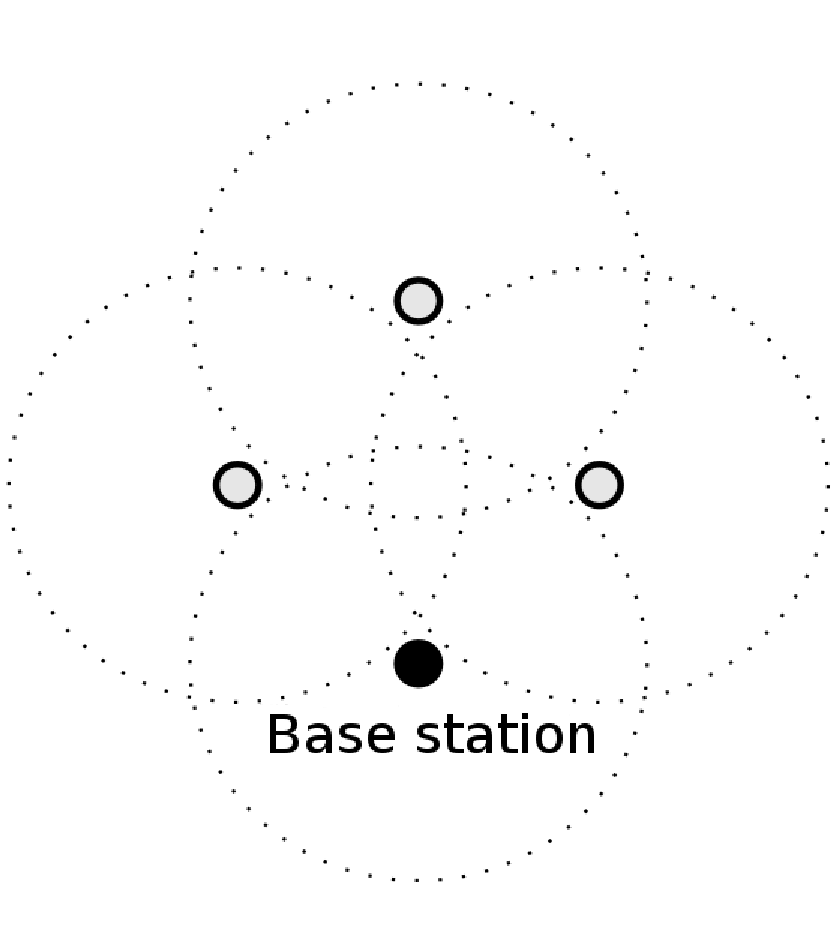
\includegraphics[scale=0.2]{fig/topology1} & 
%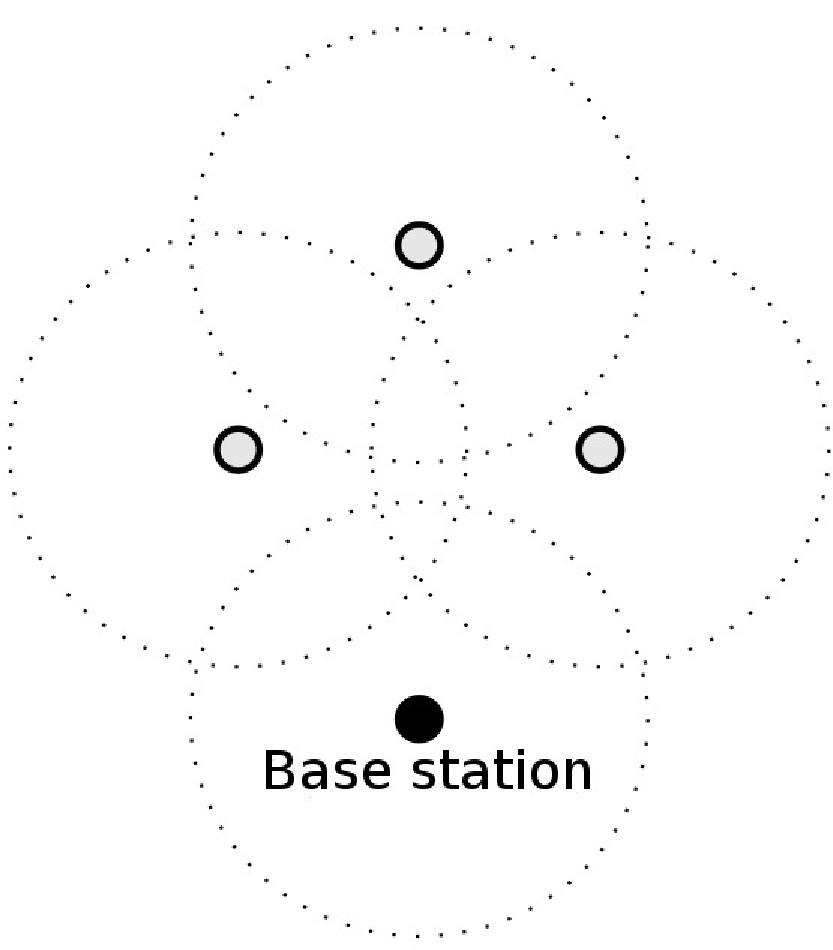
\includegraphics[scale=0.2]{fig/topology2} \\
%(a) & (b)
%\end{tabular}
%\caption{Topologies used to measure the protocol latency. (a) Base station has communication with all nodes (b) Base station does not have communication with all nodes.}
%\label{fig:topology}
%\end{figure}

%A Figura~\ref{fig:latency1} apresenta a média do tempo que a estação base leva para propagar os dados aos nodos a sua volta. Foi observado um desvio padrão de 0,0233 segundos. Este tempo não mudou alterando o número de receptores entre um e três, isto porque pacotes perdidos estão altamente correlacionados, ou seja, vários receptores perdem o mesmo conjunto de pacotes \cite{mnp}.
Figure~\ref{fig:latency1} shows the average time that the base station takes to propagate data to the nodes around it.
We observed a standard deviation of 0.0233 seconds.
This time did not change by changing the number of receivers between one and three.
This happens because loss packet is highly correlated, so multiple receivers lose the same set of packets~\cite{mnp}.

\fig{latency1}{Dissemination and reconfiguration time.}{scale=.57}

%A Figura~\ref{fig:latency2} mostra a média de tempo que os dados levam para serem propagados da estação base para nodos intermediários, e destes para o nodo fora de alcance da estação base (segunda topologia). É possível perceber que o tempo necessário para propagar dados entre nodos normais da rede é aproximadamente quatro vezes maior que o tempo gasto pela estação base, isto se deve ao fato que a estação base não executa a etapa de seleção de emissor, ou seja, não perde tempo divulgando sua versão e recebendo requisições para enfim se tornar um emissor e começar a disseminar os dados. O tempo de disseminação dos nodos intermediários apresentou um desvio padrão de 1,1288 segundos.
Figure~\ref{fig:latency2} shows the average time it takes to propagate the data from the base station to the intermediate nodes, and from these to the node out of range of the base station.
It is possible to notice that the time required to propagate data between normal network nodes is approximately four times greater than the time spent by the base station.
This is due to the fact that the base station does not perform the step of selecting a sender.
This way it wastes no time publishing its version and receiving requests to finally become a sender and begin to disseminate the data.
The time of intermediate nodes had a standard deviation of 1.1288 seconds.
 
\fig{latency2}{Dissemination time.}{scale=.57}

\subsection{Reconfiguration Time}
%Foi considerado como tempo de reconfiguração, o tempo que o nodo leva para atualizar sua memória de programa após ter recebido todos os dados necessários, via o protocolo de disseminação. Na estrutura proposta este tempo engloba: a chamada do \textsc{Reconfigurator}, os métodos \componente{p} e \componente{v} do semáforo, a chamada para o método \componente{Update}, a recuperação dos argumentos passados na mensagem ETP, a recuperação do objeto a ser atualizado em uma tabela hash, descobrir o endereço da \componente{vtable} e a escrita dos dados na flash. A Figura \ref{fig:latency1} mostra a média do tempo de reconfiguração obtido, sendo que o mesmo apresentou um desvio padrão de 0,0103 segundos.
The reconfiguration time encompasses the time a node takes to update its program memory after receiving all the necessary data.
In the proposed structure this time comprises: the call of \textsc{Reconfigurator}, methods \texttt{p} and \texttt{v} of the semaphore, the call to the \texttt{Update}, the recovery of arguments passed on the ETP message, the recovery of the object to be updated in a hash table, find the address of the \texttt{vtable}, and writing data in flash.
Figure~\ref{fig:latency1} shows the average reconfiguration time obtained. 
% It had a standard deviation of 0.0103 seconds. %%%%% isso ta errado

%Uma característica da arquitetura utilizada é que não é possível mudar apenas um byte por vez em sua memória flash. Esta memória só permite a escrita em páginas, cujo tamanho é de 256 bytes, e antes de reescrever uma página é necessário apagar seu conteúdo. Desta forma para atualizarmos uma parte da memória é necessário ler o conteúdo da página e armazená-lo em um buffer temporário, modificar apenas a parte desejada para enfim escrever na flash.
One feature of the Mica2 platform is that it is not possible to change only one byte at a time in its flash memory.
It allows only writing in pages (of 256 bytes), and before rewriting a page it is necessary to delete its contents.
Thus, in order to update a portion of memory, it is necessary to read the page content, store it in a temporary buffer, modify only the desired part of it, and finally write in the flash.
